\documentclass[a4paper, 12pt]{article}

\usepackage[UTF8]{ctex}
\usepackage[T1]{fontenc}
\usepackage[margin=2.5cm]{geometry}
\usepackage{amsmath, amssymb}
\usepackage{booktabs}
\usepackage{graphicx}
\usepackage{xcolor}
\usepackage{listings}
\usepackage{textcomp}
\usepackage{upquote}
\usepackage{titlesec}
\usepackage{fancyhdr}
\usepackage{hyperref}

\definecolor{primary}{HTML}{1F5FA8}
\definecolor{accent}{HTML}{4A90D9}
\definecolor{bgblue}{HTML}{F0F6FC}

\titleformat{\section}{\Large\bfseries\color{primary}}{\thesection}{0.8em}{}
\titleformat{\subsection}{\large\bfseries\color{accent}}{\thesubsection}{0.8em}{}

\pagestyle{fancy}
\setlength{\headheight}{14.5pt}
\fancyhf{}
\fancyhead[L]{\small\color{primary}系统开发工具基础 · 第三周实验报告}
\fancyhead[R]{\small\color{primary}陆立庭 · 25120014018}
\fancyfoot[C]{\small\color{primary}\thepage}
\renewcommand{\headrulewidth}{0.6pt}
\renewcommand{\headrule}{\color{accent}\hrule width\headwidth height\headrulewidth}

\lstset{
  basicstyle=\ttfamily\small,
  breaklines=true,
  frame=single,
  rulecolor=\color{accent},
  backgroundcolor=\color{bgblue},
  columns=fullflexible,
  upquote=true,
  showstringspaces=false,
  commentstyle=\color{gray},
  keywordstyle=\color{primary},
  stringstyle=\color{teal},
}

\hypersetup{
  colorlinks=true,
  linkcolor=primary,
  urlcolor=accent,
  citecolor=primary,
}

\title{\textbf{\color{primary}系统开发工具基础\quad 第三周实验报告}}
\author{陆立庭\ -\ 25120014018}
\date{2026 年 9 月}

\begin{document}

\maketitle
\vspace{-0.5em}
\noindent{\color{primary}\rule{\textwidth}{1pt}}

\begin{abstract}
本报告围绕第三周四个实验题目展开，覆盖 Python 包构建与分发、编程智能体的可验证修复循环、专业协作材料改写、以及 PyTorch 线性回归训练四个主题。报告按“实验题目分析与知识点总结”“实验遇到的问题与解决方法”“实验总结”“课后巩固”“GitHub 链接”五个部分组织。
\end{abstract}

\tableofcontents
\newpage

% ============================================================
\section{实验题目分析与知识点总结}
% ============================================================

\subsection{第9题：构建并验证可安装的 Python 包}

\textbf{题目分析}：采用 \texttt{src} 布局创建 \texttt{greetlab} 包，在 \texttt{pyproject.toml} 中填写自己的学号并注册 \texttt{sdt-greet} 命令；随后生成 wheel，在干净虚拟环境中只从 wheel 安装，并离开源码目录验证命令可独立运行。

\textbf{知识点}：
\begin{itemize}
  \item \texttt{src/greetlab/\_\_init\_\_.py} 用于建立可导入包，\texttt{cli.py} 提供命令入口；
  \item \texttt{[build-system]} 指定构建后端，\texttt{[project.scripts]} 把终端命令映射到 Python 函数；
  \item wheel 是可安装的二进制分发格式，使用 \texttt{python -m build} 生成；
  \item 构建环境与验证环境分离，并在 \texttt{/tmp} 中运行，可以排除从当前源码目录误导入的情况；
  \item \texttt{sha256sum} 可为构建产物生成稳定指纹，\texttt{pip show} 和 \texttt{which} 可验证包及命令来源。
\end{itemize}

核心配置与验证命令如下：

\begin{lstlisting}[language=bash]
[project]
name = "greetlab-25120014018"
version = "0.1.0"
[project.scripts]
sdt-greet = "greetlab.cli:main"

python -m build
source q09-clean-env/bin/activate
python -m pip install --no-index q09/dist/*.whl
cd /tmp
sdt-greet --name 25120014018
which sdt-greet
\end{lstlisting}

运行结果显示包版本为 0.1.0，命令输出 \texttt{Hello, 25120014018!}，且可执行文件来自 \texttt{q09-clean-env/bin}，说明 wheel 能脱离源码目录正常工作。

\begin{figure}[htbp]
  \centering
  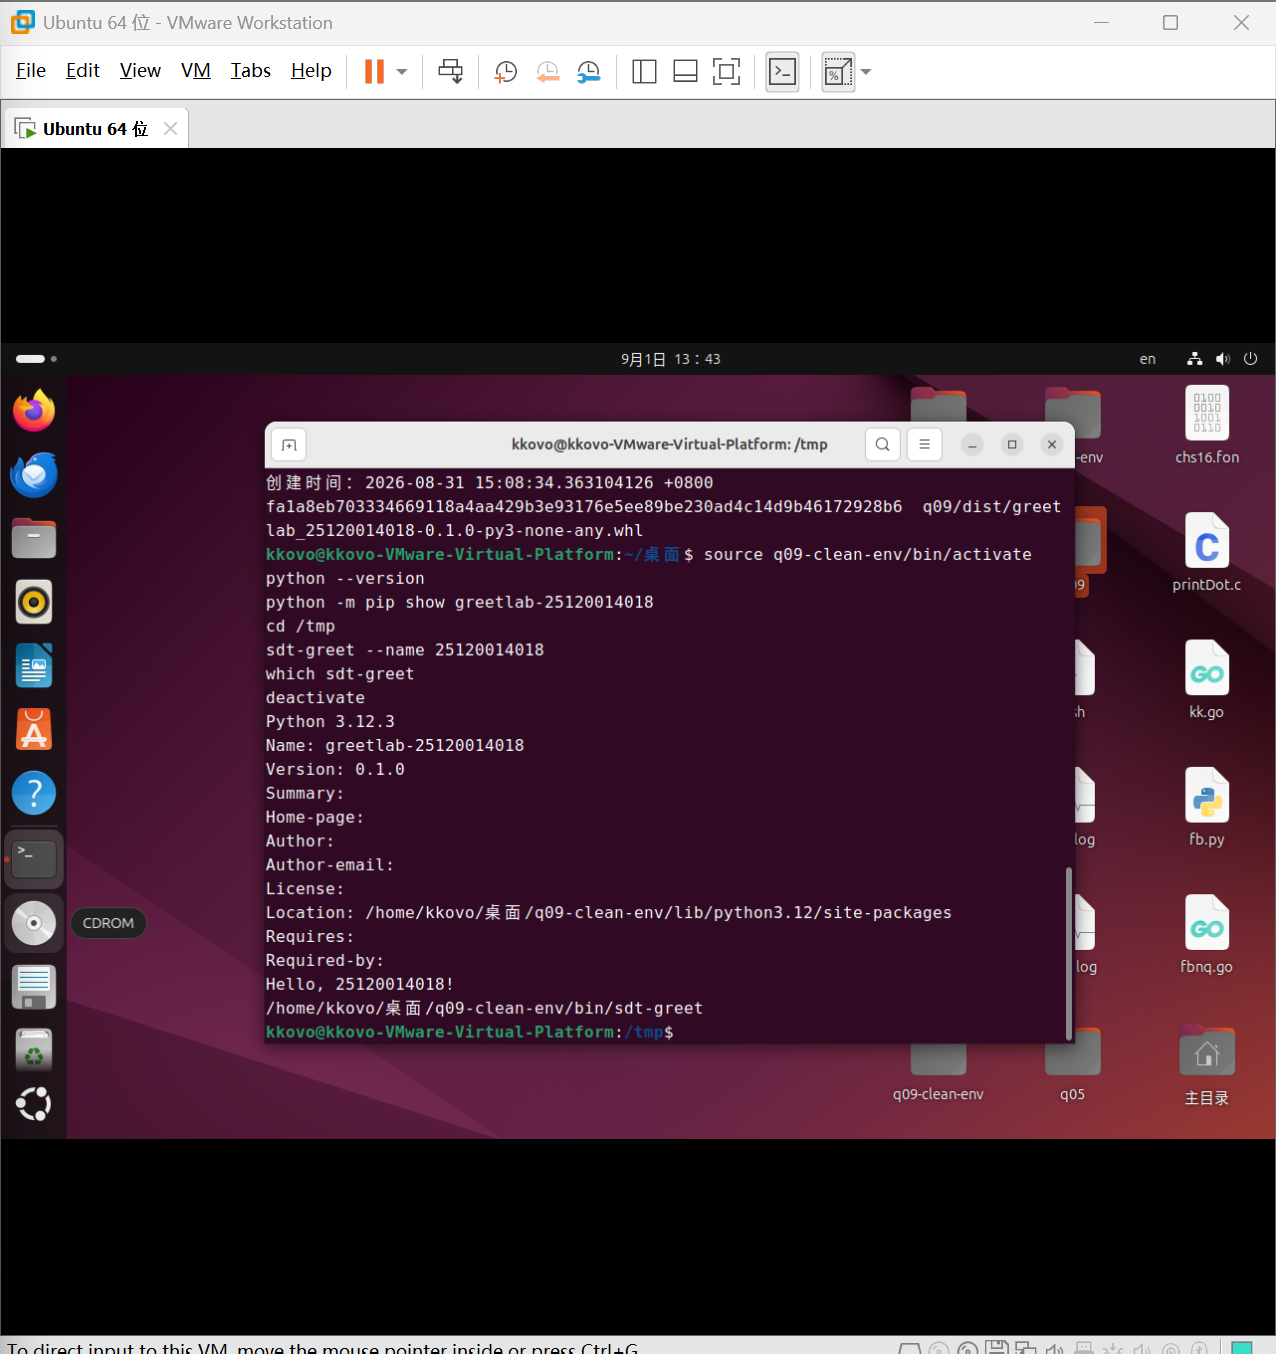
\includegraphics[width=0.88\textwidth,height=0.68\textheight,keepaspectratio]{q09.png}
  \caption{第9题：wheel 指纹、干净环境安装信息与独立运行结果}
  \label{fig:q09}
\end{figure}

\clearpage
\subsection{第10题：让编程智能体进入可验证的修复循环}

\textbf{题目分析}：为“姓名只含空白字符”添加失败测试，要求编程智能体只修改实现并运行指定测试；完成后人工检查差异、排除无关修改，再运行回归测试并在 \texttt{ai\_log.md} 中简要记录过程。

\textbf{知识点}：
\begin{itemize}
  \item 测试驱动修复遵循“先失败、再修复、最后回归”的红--绿循环；
  \item \texttt{monkeypatch} 可临时替换 \texttt{sys.argv}，\texttt{pytest.raises} 用于断言异常与退出码；
  \item \texttt{str.strip()} 将纯空白输入归一为空字符串，\texttt{argparse.ArgumentParser.error()} 会打印错误并触发 \texttt{SystemExit(2)}；
  \item 给智能体的提示应包含目标、修改范围、禁止事项和测试命令；
  \item 测试通过后仍须人工检查 diff，防止测试被篡改或出现无关重构。
\end{itemize}

关键测试与最小修复如下：

\begin{lstlisting}[language=python]
def test_blank_name_exits_2(monkeypatch):
    monkeypatch.setattr(sys, "argv", ["sdt-greet", "--name", "   "])
    with pytest.raises(SystemExit) as exc_info:
        main()
    assert exc_info.value.code == 2

# cli.py 中的最小修复
if not a.name.strip():
    p.error("name must not be blank")
\end{lstlisting}

人工核对确认实现仅增加空白姓名检查，\texttt{PYTHONPATH=src python3 -m pytest} 最终得到 \texttt{1 passed}；\texttt{ai\_log.md} 在四行内记录了提示、改动和验证。

\begin{figure}[htbp]
  \centering
  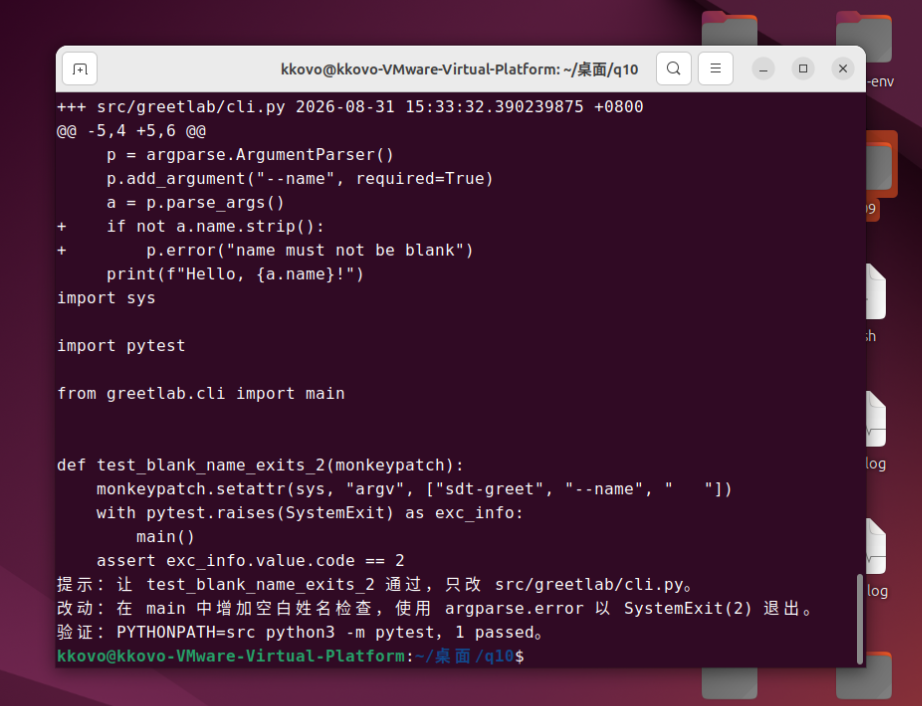
\includegraphics[width=0.88\textwidth,height=0.68\textheight,keepaspectratio]{q10.png}
  \caption{第10题：最小差异、回归测试与智能体操作记录}
  \label{fig:q10}
\end{figure}

\clearpage
\subsection{第11题：把模糊协作材料改成可执行信息}

\textbf{题目分析}：围绕“空姓名仍输出问候语”缺陷，分别重写 Issue、提交信息和评审意见。虽然文档在本地 Windows 编辑，但 Issue 描述的是缺陷发生时的 Ubuntu 运行环境，两者不能混为一谈。

\textbf{知识点}：
\begin{itemize}
  \item 可复现 Issue 至少包含环境、复现命令、期望结果和实际结果，未知信息明确标注“待确认”；
  \item 提交标题使用祈使语气，正文说明原问题与解决方案；
  \item 评审意见要指出具体行为、风险、建议动作，并使用 Blocking、Suggestion 或 Nit 标注严重程度；
  \item 协作材料的目标不是“写得长”，而是减少接收者开始处理任务前的追问成本。
\end{itemize}

本题将模糊描述改写为明确事实：执行 \texttt{sdt-greet --name " "} 时实际输出 \texttt{Hello, !} 且退出码为 0；期望行为是拒绝纯空白姓名并返回非零退出码。评审意见将该问题标记为 Blocking，并建议解析后检查 \texttt{name.strip()}，为空时调用 \texttt{p.error()}。

\begin{figure}[htbp]
  \centering
  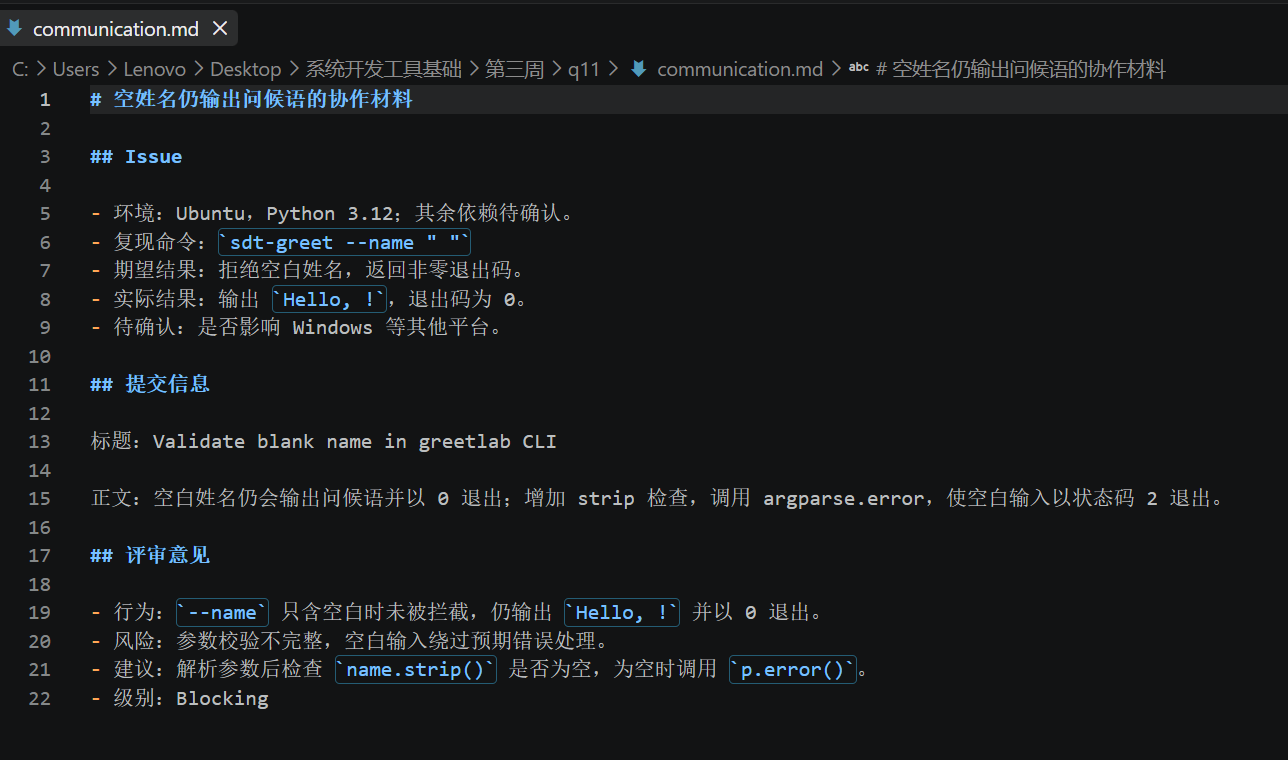
\includegraphics[width=0.92\textwidth,height=0.72\textheight,keepaspectratio]{q11.png}
  \caption{第11题：Issue、提交信息与 Blocking 评审意见}
  \label{fig:q11}
\end{figure}

\clearpage
\subsection{第12题：修复可复现的线性回归训练循环}

\textbf{题目分析}：补全 PyTorch CPU 训练循环，在不直接写死参数的前提下，使线性模型从数据中学习关系 $y=3x-1$；训练后切换评估模式，在无梯度环境中打印最终损失、weight 和 bias。

\textbf{知识点}：
\begin{itemize}
  \item \texttt{optimizer.zero\_grad()} 清除上一轮累积梯度；
  \item \texttt{loss.backward()} 根据计算图执行反向传播并计算梯度；
  \item \texttt{optimizer.step()} 按当前梯度更新模型参数；
  \item \texttt{model.eval()} 切换为评估模式，\texttt{torch.no\_grad()} 关闭梯度记录；
  \item \texttt{torch.manual\_seed} 固定初始化，使训练结果可复现。
\end{itemize}

训练循环如下：

\begin{lstlisting}[language=python]
for _ in range(200):
    pred = model(x)
    loss = loss_fn(pred, y)
    opt.zero_grad()
    loss.backward()
    opt.step()

model.eval()
with torch.no_grad():
    pred = model(x)
    loss = loss_fn(pred, y)
\end{lstlisting}

本地 PowerShell 实测最终损失为 0.000000，weight 约为 3，bias 约为 $-1$，满足误差要求。运行后计算 \texttt{train.py} 的 SHA-256，也可证明验证过程没有临时改写源码。

\begin{figure}[htbp]
  \centering
  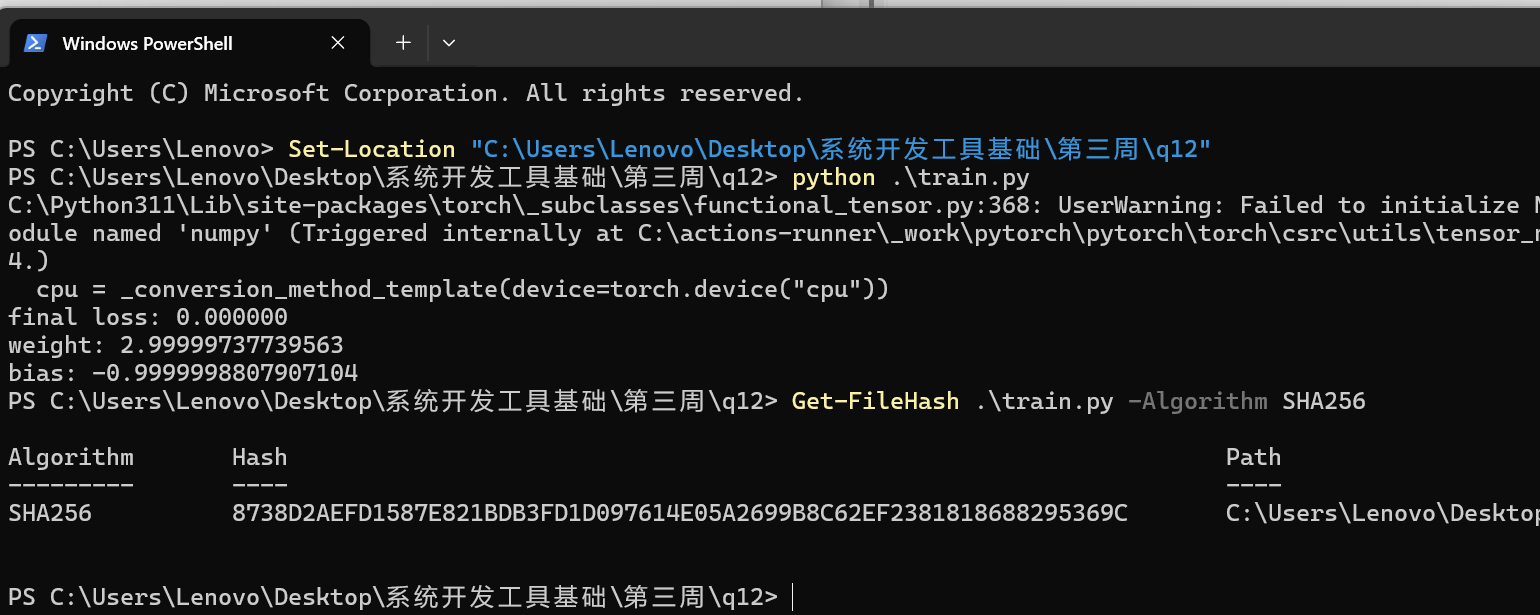
\includegraphics[width=0.92\textwidth,height=0.72\textheight,keepaspectratio]{q12.png}
  \caption{第12题：CPU 训练结果与源码 SHA-256}
  \label{fig:q12}
\end{figure}

\clearpage
% ============================================================
\section{实验遇到的问题与解决方法}
% ============================================================

\subsection{问题一：构建环境、安装环境和源码目录容易混淆}

\textbf{问题描述}：第9题同时涉及 \texttt{build-env}、\texttt{q09-clean-env} 和 \texttt{q09} 源码目录。若直接在源码目录中运行命令，即使 wheel 安装不正确，Python 也可能从当前目录找到代码，产生“看起来成功”的假象。

\textbf{解决方法}：明确分工：\texttt{build-env} 只负责执行构建，\texttt{q09-clean-env} 只从生成的 wheel 安装；激活干净环境后切换到 \texttt{/tmp} 再运行命令，并使用 \texttt{pip show}、\texttt{which} 与 SHA-256 同时验证包版本、命令来源和构建产物。

\subsection{问题二：已经修复后难以重新展示“首次测试失败”}

\textbf{问题描述}：第10题此前已经完成，当前 q10 保存的是修复后代码。如果为了截图直接把代码改坏再改回来，不但可能破坏已有成果，也不能真实代表原来的完成过程。

\textbf{解决方法}：保留 q10 的修复状态，不覆盖已有文件；人工检查 q09 与 q10 实现差异，把 q09 作为缺陷基线、q10 作为修复版本，并用测试结果、最小 diff 和 \texttt{ai\_log.md} 组成证据链。这样既能解释修复前后的行为，也不会伪造文件历史。

\subsection{问题三：文档编辑环境与缺陷运行环境容易写混}

\textbf{问题描述}：第11题的 \texttt{communication.md} 在本地 Windows 编辑，但 Issue 中的“环境”字段描述的是缺陷复现环境 Ubuntu。若直接把编辑器所在平台写入 Issue，会把“在哪里写文档”和“程序在哪里出错”混为一谈。

\textbf{解决方法}：Issue 环境只记录缺陷发生时已知的 Ubuntu、Python 3.12，并把其余依赖写为“待确认”；报告则单独说明本题文档是在本地完成。由此保持事实边界清楚，也避免猜测未知平台行为。

\subsection{问题四：PyTorch 提示无法初始化 NumPy}

\textbf{问题描述}：第12题运行时出现 \texttt{Failed to initialize NumPy: No module named 'numpy'} 警告。该警告容易被误认为训练失败，但程序随后仍输出了满足要求的 loss、weight 和 bias。

\textbf{解决方法}：先区分 warning 与异常退出。本题全部计算使用 PyTorch tensor，没有调用 tensor 与 NumPy 相互转换，因此该可选依赖警告未阻止 CPU 训练。通过最终损失与参数确认核心任务成功；若后续需要 \texttt{tensor.numpy()} 等功能，应在当前 Python 环境安装兼容版本的 NumPy 后重新运行。

% ============================================================
\section{实验总结}
% ============================================================

通过本周实验，我系统地掌握了以下内容：

\begin{itemize}
  \item \textbf{Python 包的交付链路}：能够从 src 布局、项目元数据和命令入口出发，生成 wheel，并在干净环境中验证安装结果；
  \item \textbf{智能体修复的验证意识}：理解提示词不能只说“修 bug”，而要约束修改范围、给出测试命令，并在智能体完成后人工检查 diff；
  \item \textbf{专业协作表达}：能够把模糊 Issue、提交信息和评审意见改写为接收者可以直接执行的信息；
  \item \textbf{PyTorch 基础训练流程}：掌握清梯度、反向传播、参数更新，以及训练模式与评估模式的区别。
\end{itemize}

本周四题看似分别属于打包、智能体、沟通和机器学习，实际贯穿了同一条工程原则：结果必须可交付、可复现、可验证。能运行一次并不等于完成；还需要证明运行的是正确产物、修复没有无关改动、文字能让协作者复现、训练结果来自优化过程而不是写死参数。

% ============================================================
\section{课后巩固：12 个实例练习}
% ============================================================

为巩固本周四道题的知识点，我另外设计了 12 个由浅入深的新实例。实例 1～6 在 Ubuntu 虚拟机完成，实例 7～12 在本地 Windows 完成；每个实例均按“练什么 $\rightarrow$ 任务 $\rightarrow$ 思路 $\rightarrow$ 参考 $\rightarrow$ 自查”的流程组织。

\begin{table}[htbp]
  \centering
  \small
  \begin{tabular}{cllp{6.1cm}}
    \toprule
    \textbf{\#} & \textbf{实例} & \textbf{主题} & \textbf{覆盖知识点} \\
    \midrule
    1 & 认识 src 布局 & Python 打包 & 包目录、模块导入 \\
    2 & 注册 score-badge 命令 & Python 打包 & pyproject、命令入口 \\
    3 & wheel 独立安装 & Python 打包 & build、虚拟环境 \\
    4 & 先写失败测试 & 智能体编程 & pytest、SystemExit \\
    5 & 写清智能体提示 & 智能体编程 & 目标、约束、验证 \\
    6 & 人工检查修复 & 智能体编程 & diff、回归测试 \\
    7 & 写可复现 Issue & 协作材料 & 环境、复现、期望、实际 \\
    8 & 写规范提交信息 & 协作材料 & 祈使语气、问题与方案 \\
    9 & 写评审意见 & 协作材料 & 行为、风险、动作、级别 \\
    10 & 创建训练数据 & PyTorch & tensor、reshape \\
    11 & 观察一次参数更新 & PyTorch & 梯度与优化器 \\
    12 & 完整可复现训练 & PyTorch & train/eval、no\_grad \\
    \bottomrule
  \end{tabular}
  \caption{第三周课后巩固的 12 个实例总览}
  \label{tab:practice3}
\end{table}

\subsection{解题感悟}

课后把这 12 个实例按顺序敲下来后，我对“验证”有了更具体的认识。以前我容易把“终端有输出”当作完成，但打包练习让我发现，如果不离开源码目录，就不能证明 wheel 真的安装正确；智能体修复也一样，只有先看到测试失败、再看到修复后通过，并亲自检查 diff，才知道智能体解决的是原问题而不是绕过测试。协作材料练习让我体会到，Issue 写清楚环境、命令和实际结果，本身就是在节省团队时间。PyTorch 的三步练习则把原来抽象的反向传播拆成了可观察的梯度和参数变化。相比单纯记命令，这种一步一步验证的过程更容易形成长期记忆。

完整版（含每个实例的思路与参考代码）保存在配套的《第3周 12 个实例练习》Markdown 文档中，可随课程仓库一并提交。

% ============================================================
\section{附录：GitHub 链接与提交记录}
% ============================================================

本次实验代码已提交至课程 GitHub 仓库：

\begin{center}
  \url{https://github.com/lyun69965/primary-system-tools.git}
\end{center}

第9至12题分别建立了内容聚焦的独立提交，提交记录如下图所示：

\begin{figure}[htbp]
  \centering
  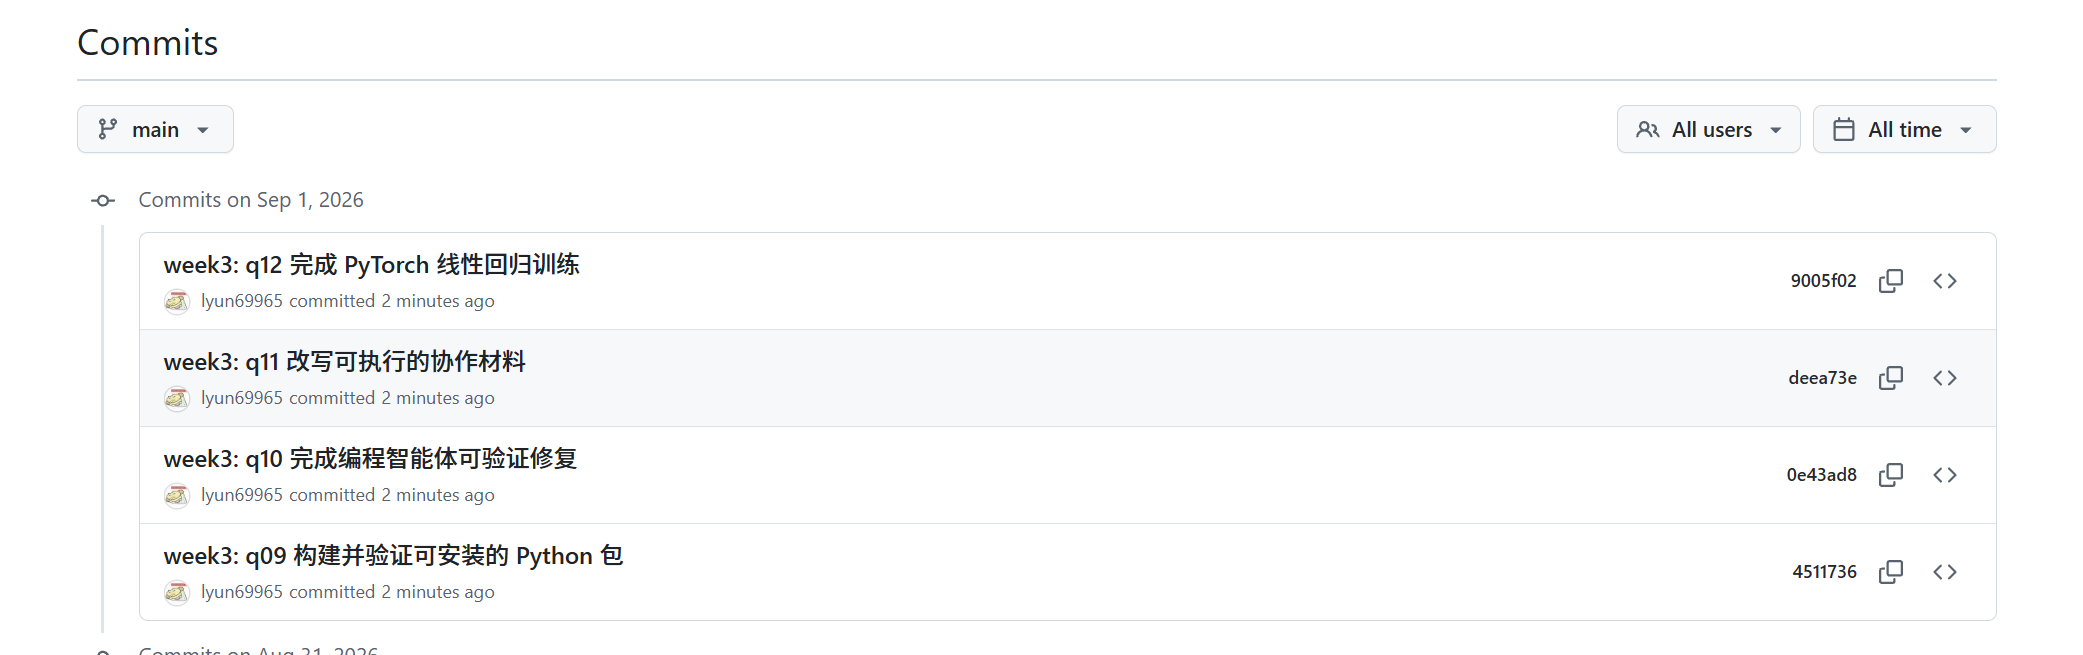
\includegraphics[width=0.94\textwidth,height=0.62\textheight,keepaspectratio]{commit_week3.png}
  \caption{第三周第9至12题的 GitHub commit 提交记录}
  \label{fig:commit3}
\end{figure}

\end{document}
